\documentclass[twocolumn]{aastex63}

\usepackage{float}
\graphicspath{{./}{figures/}}

\newcommand{\vdag}{(v)^\dagger}
\newcommand\aastex{AAS\TeX}
\newcommand\latex{La\TeX}

\shorttitle{H-R Diagram Project}
\shortauthors{C. Gobat}

\begin{document}

\title{\Large{Using SDSS Data and Python in the Compilation and Composition of a Hertzsprung-Russell Diagram}}


\author[0000-0003-1268-8845]{Caden Gobat}
\affiliation{Department of Physics \\ The George Washington University \\ Washington, DC 20052, USA}
\email{cgobat@gwu.edu}
\collaboration{1}{(PHYS 2023, Fall 2019)}

\author[0000-0002-5422-4873]{Kalvir S. Dhuga}
\affiliation{Department of Physics \\ The George Washington University \\ Washington, DC 20052, USA}
\email{dhuga@gwu.edu}
\collaboration{1}{(Advising Professor)}


\begin{abstract}

The Hertzsprung-Russell (H-R) diagram is a foundational visualization tool of modern astronomy that plots stars' luminosity against their temperature, spectral class, or color (all essentially synonymous). Here I make use of stellar spectral and parallax data collected by the Sloan Digital Sky Survey to fit and plot a representative H-R diagram using Python and  Matplotlib. The result is a high-precision, visually appealing graphic, which is presented here, along with the methods used to generate it.

\end{abstract}

\keywords{astronomical databases: miscellaneous --- methods: data analysis --- Hertzsprung–Russell and C–M diagrams --- stars: luminosity function, mass function}


\section{Introduction} \label{sec:intro}

Although the study of the stars on the whole is a practice that dates back millennia, the characterization of patterns and relationships among their spectra and other properties began to be truly solidified at the beginning of the twentieth century with works such as \citet{Hertzsprung_1911} and \citet{Norris_1912}, who plotted stars' luminosities against their colors and temperatures. Doing so brings to light a number of revelations about stellar classification (main sequence, dwarfs, giants, etc.), life cycles, and a multitude of other insights.

In order to create such a diagram, the provided observational data from the Sloan Digital Sky Survey \citep{SDSS-IV} was imported and processed using a series of Python algorithms implemented by the author. Python was chosen over a more simplistic software such as Excel or Google Sheets because it provides more precision and automation in the handling of the data, especially for large datasets. Using packages such as Pandas \citep{pandas} and astropy \citep{astropy} allows for greater control in the manipulation of the data as well as a more readily scalable method to analyze much larger datasets. Overall, the use of Python is a more advanced, robust technique that is much more efficient than manual spreadsheet computations on large datasets. Additionally,  Matplotlib \citep{matplotlib} enables a much higher degree of control over visualizations and plots of the data than most spreadsheet programs.

\section{Data Collection \& Parsing} \label{sec:data}

Data on stellar properties was provided in two separate catalog excerpt files: one main list (\verb|HR-project-stars(1).xlsx|), which included stars from a variety of spectral and luminosity classes, and one that contained exclusively white dwarfs (\verb|wd-stars.xlsx|). For the main list of stars, data was provided for the following variables: apparent magnitude in the V band, right ascension, declination, parallax angle, B-V color, and spectral class. The white dwarfs list contains all of the same information categories, with the addition of a column containing absolute magnitude in the V band as well.

Because the primary list did not contain information about the absolute magnitudes of the stars, it was necessary to calculate using apparent magnitude and distance. Because an object's apparent brightness is a function of both how bright it actually is and how far away it is, knowing two of these values allows for the calculation of the third. In this case, the formula for performing this conversion to absolute visual magnitude (${\verb|M|}_{\verb|V|}$) is given in Eq. (\ref{eq:absmag}), where \verb|par| is the measured parallax angle in milliarcseconds and \verb|Vmag| is the apparent visual magnitude.

\begin{equation} \label{eq:absmag}
  \text{M}_{\text{V}} = \text{Vmag} + 5\times\log(\frac{\text{par}}{100})
\end{equation}

In order to execute this calculation, and the rest of the procedures described here, the two spreadsheets were converted into .csv format in order to be loaded into a Python environment through the Pandas module for analysis. After generating an ${\verb|M|}_{\verb|V|}$ column for the main list, the two datasets contained all of the same variables, and could be compiled into one master catalog. Each column of the white dwarfs list was appended to the corresponding column of the main list. Then, absolute luminosities could be calculated for all of the stars using Eq. (\ref{eq:luminosity}) (provided).

\begin{equation} \label{eq:luminosity}
    \text{L}/\text{L}_\odot = 2.512^{4.83-\text{M}_{\text{V}}}
\end{equation}

With this, the dataset now contains all of the information necessary for the creation of the diagram.

\section{Color \& Temperature} \label{sec:colortemp}

One of the major breakthroughs of the early twentieth century was the characterization of the black-body radiation spectrum. This revealed that a black-body radiator (such as a star) has a color that is directly related to its temperature. Given that the color index of each star is provided in the dataset (B--V index, the magnitude in the V band subtracted from that in the B band---referred to as \verb|BV| for convenience), their temperatures can be inferred. First, a model must be developed that relates the two variables numerically. To this end, a calibration dataset of empirical observations of color and temperature for 14 objects was provided (\verb|stars-color-color-diagrams.xls|).

The following equation was initially suggested to fit the color-temperature calibration data:
\begin{eqnarray} \label{eq:a-poly}
  \log{T} = a_0 + a_1(\text{BV}) + a_2(\text{BV})^2 \nonumber\\ + a_3(\text{BV})^3 + a_4(\text{BV})^4
\end{eqnarray}

\newpage

With provided coefficient weights of:
\begin{eqnarray*}
a_0 &=& +3.986; \\ a_1 &=& -0.558; \\ a_2 &=& +0.498; \\ a_3 &=& -0.324; \\ a_4 &=& +0.078
\end{eqnarray*}

As a check, a non-linear least-squares fit was performed to optimize the \emph{a} coefficients This yielded a model that overfit the data, making the coefficients deviate significantly from the originals.

However, the accepted\footnote{implemented in packages such as \href{https://github.com/sczesla/PyAstronomy}{PyAstronomy}} formula is given in Eq. (\ref{eq:ballesteros}), and was first presented by \citet{Ballesteros_2012}, who derived it by considering stars as black-bodies, which is a fairly appropriate approximation for most purposes. 

\begin{equation} \label{eq:ballesteros}
  T = 4600\text{ K}(\frac{1}{0.92(\text{BV})+1.7}+\frac{1}{0.94(\text{BV})+0.62})
\end{equation}

All three of these fits are plotted in Fig. (\ref{fig:colortemp}), which shows that the accepted model is actually reproduced more closely by the original polynomial coefficients, rather than the optimized ones. This is likely because the fitting engine attempted to overly compensate for erroneous fluctuations in the data, making it actually less reflective of the real relationship.

\begin{figure}[!h]
\centering
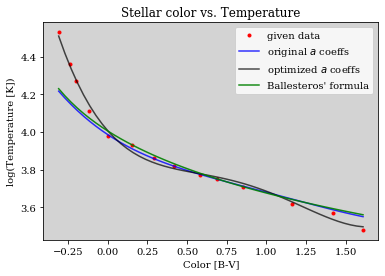
\includegraphics[width=\linewidth]{colortemps.png}
\caption{The various fits between color and temperature of several exemplar stars (data plotted in red). The blue line plots the fourth-order polynomial (Eq. \ref{eq:a-poly}) using the given \emph{a}-coefficients. The black uses the optimized coefficient weights, and shows an obvious discrepancy between the original and fitted polynomials. The green line shows that the accepted formula derived from black-body radiation theory is much more in line with the original model than the fitted one.
\label{fig:colortemp}}
\end{figure}

Given the close similarity between the original-coefficient fourth-order polynomial and Ballesteros' formula (on this domain, anyway), it does not particularly matter which is used for the rest of the analysis.

Now, with a model to convert between B-V color index and temperature, the surface temperature of each star in the catalog can be determined.

\section{The H-R Diagram: Results and Conclusions} \label{sec:HR}

There are essentially three different variables that can be used as the horizontal axis of an H-R diagram: color index, temperature, and spectral class. All of these values are essentially synonymous, and converting between them is a simple task. For the purposes of this diagram, all three were used in some way. The data were originally plotted using the color index as the abscissa and luminosity as the ordinate. Then, temperatures were matched with these colors (using the formulas described previously) and charted on a secondary horizontal axis at the top of the diagram. Finally, the labels on the main x-axis were replaced by the spectral classes (O, B, A, F, G, K, M) at their respective locations and color index was denoted using a scaled color scheme, keyed using a colorbar on the right of the diagram.

The Python code block used to generate the plot itself out of the formatted data is provided in Fig. (\ref{fig:plotcode}), with a link to the complete source code used for analysis in Appendix \ref{sec:links} (readers are encouraged to follow the link to gain a full appreciation for how the code works). The finished product itself is presented in Fig. (\ref{fig:HRdiagram}), as generated by the Matplotlib code shown. Both figures appear on the following page.

\begin{figure*}[!h]
    \centering
    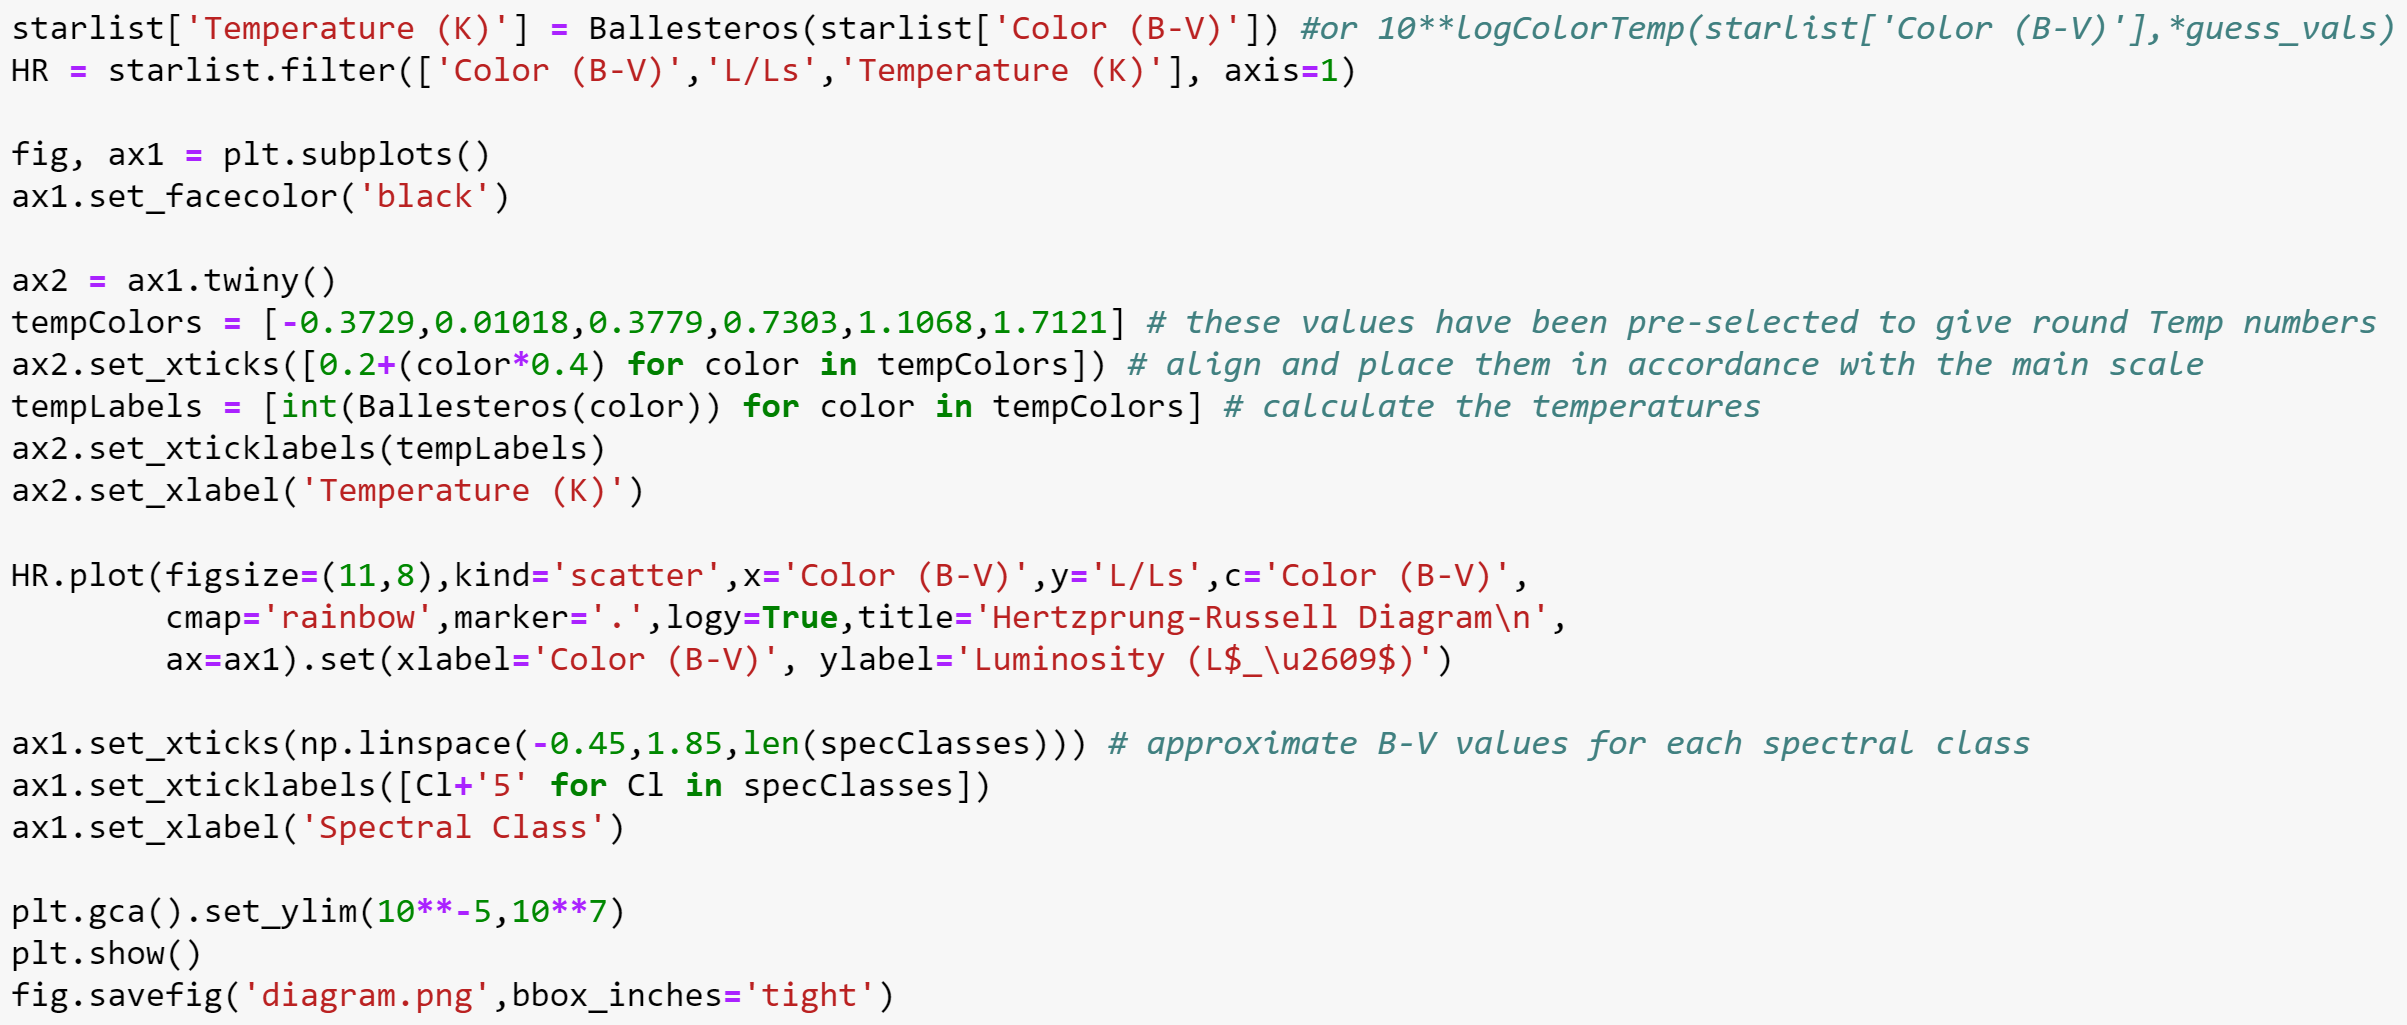
\includegraphics[width=0.8\textwidth]{graph_code.png}
    \caption{Once the data were analyzed, this code block generates and saves the H-R diagram as it appears below.}
    \label{fig:plotcode}
\end{figure*}

\begin{figure*}[!h]
  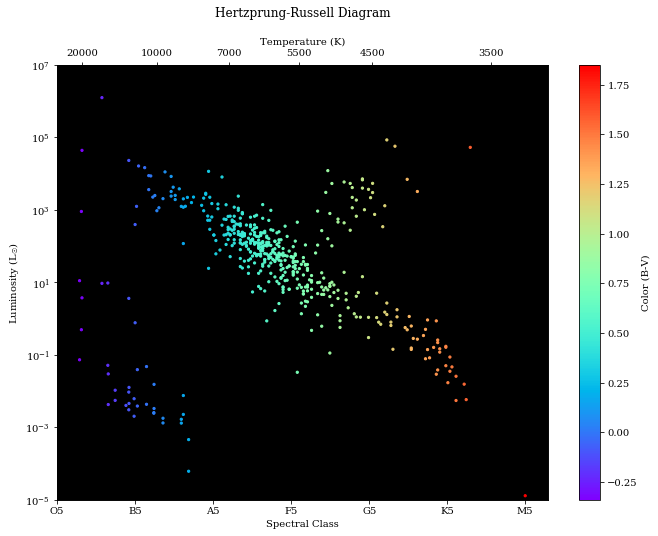
\includegraphics[width=0.9\textwidth]{diagram.png}
  \caption{The H-R diagram created using the data provided for this project. On the bottom horizontal axis is the approximate spectral class, while the top denotes corresponding effective temperatures. On the horizontal axis is the stars' luminosities in units of solar luminosities, on a logarithmic scale. The colorbar to the right provides information as to the B-V color index of each star, which is essentially another measure of surface temperature.}
  \label{fig:HRdiagram}
\end{figure*}

In general, the creation of the H-R diagram was a success, as the groups that one expects to appear indeed reveal themselves: there is a clear main sequence spanning the plot from upper left to lower right, with a distinctly separate group of dwarfs to the lower left. The giants branch also extends upward and to the right from the main sequence, as it should.

This project confirmed the empirical nature of the relationships displayed on H-R diagrams, and provided a valuable exercise in computational analysis of real observational data.

\acknowledgments

This research made use of Astropy, a community-developed core Python package for Astronomy.

Funding for the Sloan Digital Sky Survey IV has been provided by the Alfred P. Sloan Foundation, the U.S. Department of Energy Office of Science, and the Participating Institutions. SDSS-IV acknowledges support and resources from the Center for High-Performance Computing at the University of Utah. The SDSS web site is \url{www.sdss.org}. SDSS-IV is managed by the Astrophysical Research Consortium for the \href{https://www.sdss.org/collaboration/affiliations/}{Participating Institutions of the SDSS Collaboration}.

This report was typeset using AAS\TeX{} v6.3, a resource provided by the \href{https://journals.aas.org/aastex-package-for-manuscript-preparation/}{American Astronomical Society}.

\facilities{SDSS}

\software{Python, pandas,  Matplotlib, astropy}

\bibliography{sample63}{}
\bibliographystyle{aasjournal}

\appendix
\section{Sky Chart} \label{sec:skymap}

For reference purposes, astropy and  Matplotlib were used to create a visualization of the locations of the given stars using the provided right ascension and declination information.

\begin{figure}[!h]
    \centering
    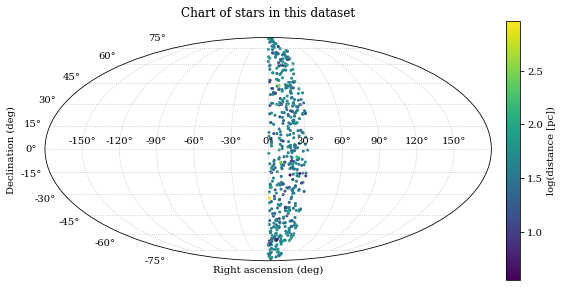
\includegraphics[width=\textwidth]{skymap.png}
    \caption{A Mollweide projection of the sky with the stars in this dataset charted. The points' colors correspond to their distances from Earth.}
    \label{fig:skymap}
\end{figure}

It is noteworthy that stars in this excerpt are shown to all be located between 0$^{\circ}$ and 30$^{\circ}$ of right ascension, spanning the full $\pm90^{\circ}$ of declination. Additionally, the color mapping shows that most stars are located at a distance on the order of $\sim$$10^1$ to $10^2$ parsecs away.

\section{Reference Links} \label{sec:links}

\begin{itemize}
    \item \href{https://drive.google.com/file/d/1skbQMEpihvruBT3py0GIvwL7lylB5EGR/view?usp=sharing}{Complete source code} - Jupyter or \href{https://colab.research.google.com/}{Colab} notebook \citep[requires IPython:][]{IPython}
    \item \href{https://blackboard.gwu.edu/bbcswebdav/pid-9747006-dt-content-rid-65358190_2/xid-65358190_2}{Main list of stellar data} (accessible to PHYS 2023 course members only)
    \item \href{https://blackboard.gwu.edu/bbcswebdav/pid-9747009-dt-content-rid-65358195_2/xid-65358195_2}{List of white dwarf data} (accessible to PHYS 2023 course members only)
    \item \href{https://blackboard.gwu.edu/bbcswebdav/pid-9747011-dt-content-rid-65358198_2/xid-65358198_2}{Star color-temperature calibration data} (accessible to PHYS 2023 course members only)
    \item \href{https://skyserver.sdss.org/dr15/en/proj/advanced/hr/hrhome.aspx}{Information on the H-R diagram provided by SDSS}
\end{itemize}


\end{document}